\documentclass[a4paper,12pt]{article}

%%% Работа с русским языком
\usepackage{cmap}					% поиск в PDF
\usepackage{mathtext} 				% русские буквы в формулах
\usepackage[T2A]{fontenc}			% кодировка
\usepackage[utf8]{inputenc}			% кодировка исходного текста
\usepackage[english,russian]{babel}	% локализация и переносы
\usepackage{xcolor}
\usepackage{hyperref}
 % Цвета для гиперссылок
\definecolor{linkcolor}{HTML}{799B03} % цвет ссылок
\definecolor{urlcolor}{HTML}{799B03} % цвет гиперссылок

\hypersetup{pdfstartview=FitH,  linkcolor=linkcolor,urlcolor=urlcolor, colorlinks=true}

%%% Дополнительная работа с математикой
\usepackage{amsfonts,amssymb,amsthm,mathtools} % AMS
\usepackage{amsmath}
\usepackage{icomma} % "Умная" запятая: $0,2$ --- число, $0, 2$ --- перечисление

%% Номера формул
%\mathtoolsset{showonlyrefs=true} % Показывать номера только у тех формул, на которые есть \eqref{} в тексте.

%% Шрифты
\usepackage{euscript}	 % Шрифт Евклид
\usepackage{mathrsfs} % Красивый матшрифт

%% Свои команды
\DeclareMathOperator{\sgn}{\mathop{sgn}}

%% Перенос знаков в формулах (по Львовскому)
\newcommand*{\hm}[1]{#1\nobreak\discretionary{}
{\hbox{$\mathsurround=0pt #1$}}{}}
% графика
\usepackage{graphicx}
\graphicspath{{pictures/}}
\DeclareGraphicsExtensions{.pdf,.png,.jpg}
\author{Бурмашев Григорий, БПМИ-208}
\title{ТВиМС, дз -- 3}
\date{\today}
\begin{document}
\maketitle
\clearpage
\section*{Номер 11 [лист 1]}
\begin{center}
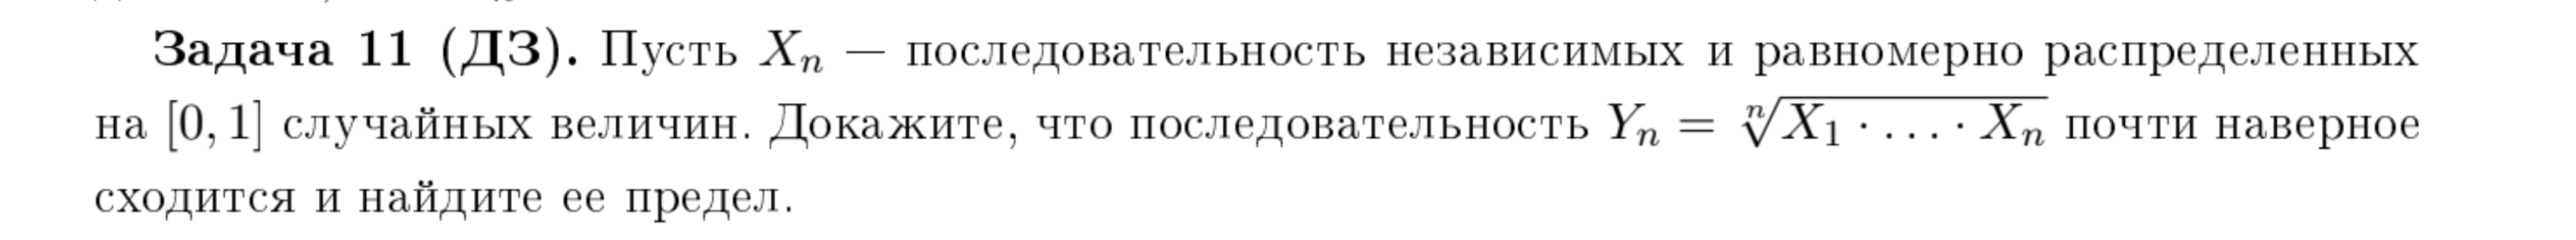
\includegraphics[scale=0.3]{1.png}
\end{center}
От Зеленова была подсказка про закон больших чисел, попробуем подвести под него. Посмотрим на $\ln X_n$:
\[
\forall n \in \mathbb{N} \; : \; \mathbb{E} \left( \ln (X_n)  \right)= \int_{-\infty}^{+\infty} \ln x \rho(x) dx = \int_{0}^{1} \ln x dx  =
x \cdot \left(\ln x - 1 \right) \Bigg|_0^2
= -1
\]
Теперь смотрим на $Y_n$:
\[
\ln \sqrt[n]{X_1 \cdot \ldots \cdot X_n} = \frac{1}{n} \cdot \ln (X_1 \cdot \ldots \cdot X_n) = \frac{1}{n} \cdot \ln(X_1) \cdot \ldots \cdot \ln (X_n) = \frac{\ln(X_1) \cdot \ldots \cdot \ln (X_n)}{n}
\]
По уЗБЧ Колмогорова это стремится к $\mathbb{E} \ln(X_1)$, что равно -1. Тобишь:
\[
\ln (Y_n) \overset{\text{п.н}}{\longrightarrow} -1
\]
Отсюда:
\[
Y_n \overset{\text{п.н}}{\longrightarrow} e^{-1}
\]
\begin{center}
\textbf{Ч.Т.Д } 
\end{center}
\clearpage
\section*{Номер 2 [не из листа]}
\begin{center}

\includegraphics[scale=0.4]{2.png}
\end{center}
\subsection*{a)}
По определению хотим:
\begin{center}
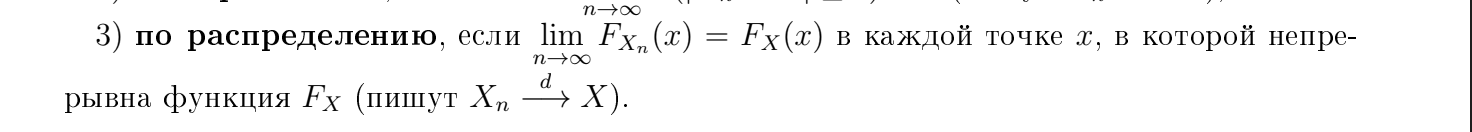
\includegraphics[scale=0.4]{4.png}
\end{center}
Смотрим на функцию распределения
\[
F_{X_n}(t) = P(X_n \leq t) = 
\begin{cases}
1, t \geq 2 \\
\frac{1}{2}, t \in [1, 2) \\
0,  \text{иначе}
\end{cases}
\]
А для $X_1$ (т.к условия нашей последовательности выполняется для любого $n$):
\[
F_{X_1}(t) = P(X_1 \leq t) = 
\begin{cases}
1, t \geq 2 \\
\frac{1}{2}, t \in [1, 2) \\
0,  \text{иначе}
\end{cases}
\]
Как не сложно заметить, они равны в каждой точке $t$, в которой непрерывна функция $F_{X_1}$. Ну в таком случае $F_{X_n}$ стремится при $n \rightarrow \infty$ к $F_{X_1}$, а значит:
\[
X_n \overset{d}{\longrightarrow} X_1
\]
\begin{center}
\textbf{Ч.Т.Д} 
\end{center}

\subsection*{b)}
По определению смотрим на отрицание сходимости по вероятности
\[
\exists \varepsilon > 0 \; : \; 
\lim_{n \rightarrow \infty} P
(
\left|
X_n - X_1
\right|
\geq \varepsilon
)
\neq 0 
\; ?
\] 
 Посмотрим на нашу последовательность. $X_i$ принимает значения либо 1, либо 2. Если случится, что $X_n$ и $X_1$ примут разные значения, то при $\varepsilon = 1$ выполнится отрицание. Заметим, что:
\[
P(X_n = X_1) = \frac{1}{2}
\]
Потому что всего у нас 4 возможных исхода (1 1, 2 2, 1 2, 2 1), и подходят из них нам только два. В таком случае:
\[
P(X_1 \neq X_1) = 1 - P(X_n = X_1) = \frac{1}{2}
\]
Теперь можем зафиксировать $\varepsilon = 1$ и получить:
\[
\lim_{n \rightarrow \infty} P
(
\left|
X_n - X_1
\right|
\geq \varepsilon
)
=
\lim_{n \rightarrow \infty} P
(
\left|
X_n - X_1
\right|
\geq 1
)
=
P(X_n \neq X_1)
=
\frac{1}{2}
\neq 0 
\]
Выполнилось отрицание, а значит:
\[
X_n \overset{P}{\nrightarrow} X_1
\]
\begin{center}
\textbf{Ч.Т.Д} 
\end{center}
Теперь проверяем сходимость в среднем квадратичном. По определению:
\begin{center}
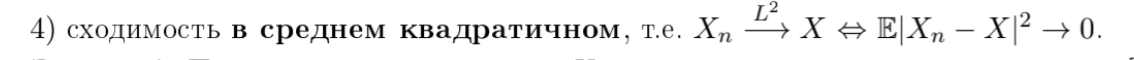
\includegraphics[scale=0.5]{5.png}
\end{center}
Смотрим на это мат.ожидание. Посмотрим, какие значения может принимать $|X_n - X_1|$:
\begin{center}
\begin{tabular}{|c|c|c|}
\hline
$X_n / X_1$& 1 & 2 \\
\hline
1 & 0 & 1 \\
\hline
2 & 1 & 0 \\
\hline
\end{tabular}
\end{center}
Тогда распределение:
\begin{center}
\begin{tabular}{|c|c|c|c|}
\hline
 $|X_n - X|$& 0 &1 \\
\hline
 $P$&  $\frac{1}{2}$& $\frac{1}{2}$ \\
\hline
\end{tabular}
\end{center}
Отсюда получаем:
\[
\mathbb{E} 
\left|
X_n - X
\right|^2 
=
0 \cdot \frac12 + 1 \cdot \frac12 = \frac12 \neq 0
\]
А значит нет стремления к нулю, следовательно и нет сходимости в среднем квадратичном, т.е:
\[
X_n \overset{L_2}{\nrightarrow} X_1
\]
\begin{center}
\textbf{Ч.Т.Д} 
\end{center}
\end{document}
